The final held-out comparison is complete. Table~\ref{tab:test} reports all 206 annotations from the reserved eight patients. Original and adapted phases use the same frozen base, quantization, prompt, greedy decoding and automatic SDPA; the adapter is disabled only for the original phase. The returned predictions were independently checked against the original source inputs and expert targets, re-parsed with the frozen strict parser, and all classification/evidence metrics were recomputed. No subsequent tuning is performed.
\begin{table*}[t]\centering\small\caption{Final held-out test results, separate from development validation.}\label{tab:test}\begin{tabular}{llrrrr}
\toprule
Group & Model & N & Accuracy & Macro F1 & Evidence F1 \\
\midrule
overall & before & 206 & 0.4078 & 0.3492 & 0.4571 \\
inclusion & before & 75 & 0.7067 & 0.5815 & 0.5524 \\
exclusion & before & 131 & 0.2366 & 0.1905 & 0.1714 \\
overall & after & 206 & 0.7427 & 0.4733 & 0.5714 \\
inclusion & after & 75 & 0.7600 & 0.5802 & 0.6847 \\
exclusion & after & 131 & 0.7328 & 0.3508 & 0.2222 \\
\bottomrule
\end{tabular}
\end{table*}
Accuracy improves from 0.4078 (84/206) to 0.7427 (153/206), a gain of 33.50 percentage points. Overall macro-F1 rises from 0.3492 to 0.4733. Inclusion accuracy increases from 0.7067 to 0.7600, but inclusion macro-F1 falls slightly from 0.5815 to 0.5802. Exclusion accuracy rises from 0.2366 to 0.7328 and macro-F1 from 0.1905 to 0.3508. Both phases produce valid JSON/categories/citations for every test record; validity is not the same as clinical correctness.

Table~\ref{tab:testclasses} preserves every applicable category and zero-support class. The not-excluded category improves from 2/91 to 89/91 correct, explaining much of the aggregate gain. Not-included recall falls from 3/7 to 1/7, while not-applicable recall falls from 11/15 to 3/15. Included recall is unchanged at 20/27. These regressions prevent describing adaptation as uniformly better. There are no gold excluded examples in this test group, so excluded sensitivity cannot be estimated; its zero score remains in the fixed applicable macro-F1 rather than silently removing the class.
\begin{table*}[t]\centering\footnotesize\caption{Final test category metrics overall and by criterion type. P/R/F1 denotes precision/recall/F1; zero-support classes remain.}\label{tab:testclasses}\begin{tabular}{lrrr}
\toprule
Group / category & N & Before P/R/F1 & After P/R/F1 \\
\midrule
overall / included & 27 & 0.909/0.741/0.816 & 0.909/0.741/0.816 \\
overall / not included & 7 & 0.300/0.429/0.353 & 0.333/0.143/0.200 \\
overall / excluded & 0 & 0.000/0.000/0.000 & 0.000/0.000/0.000 \\
overall / not excluded & 91 & 1.000/0.022/0.043 & 0.736/0.978/0.840 \\
overall / not enough information & 66 & 0.369/0.727/0.490 & 0.702/0.606/0.650 \\
overall / not applicable & 15 & 0.268/0.733/0.393 & 1.000/0.200/0.333 \\
inclusion / included & 27 & 0.909/0.741/0.816 & 0.909/0.741/0.816 \\
inclusion / not included & 7 & 0.300/0.429/0.353 & 0.333/0.143/0.200 \\
inclusion / not enough information & 38 & 0.778/0.737/0.757 & 0.714/0.921/0.805 \\
inclusion / not applicable & 3 & 0.286/0.667/0.400 & 1.000/0.333/0.500 \\
exclusion / excluded & 0 & 0.000/0.000/0.000 & 0.000/0.000/0.000 \\
exclusion / not excluded & 91 & 1.000/0.022/0.043 & 0.736/0.978/0.840 \\
exclusion / not enough information & 28 & 0.213/0.714/0.328 & 0.625/0.179/0.278 \\
exclusion / not applicable & 12 & 0.265/0.750/0.391 & 1.000/0.167/0.286 \\
\bottomrule
\end{tabular}
\end{table*}
Evidence micro-F1 improves from 0.4571 to 0.5714. Adapted micro precision is 0.7925 and recall 0.4468 (42 true positives, 11 false positives and 52 false negatives). Table~\ref{tab:testevidence} includes micro/macro precision, recall and F1, with nonempty-gold-only F1. Of 206 records, 145 have empty gold evidence; consequently macro-F1 of 0.8343 substantially exceeds the nonempty-only value of 0.5553. Exclusion evidence recall is only 0.1250, so improved label accuracy must not obscure weak support retrieval.
\begin{table*}[t]\centering\scriptsize\caption{Final held-out evidence metrics with the explicit empty-set policy. Nonempty F1 is example-macro F1 restricted to nonempty gold.}\label{tab:testevidence}\begin{tabular}{llrrrrrrr}
\toprule
Group & Model & Micro P & Micro R & Micro F1 & Macro P & Macro R & Macro F1 & Nonempty F1 \\
\midrule
overall & before & 0.6957 & 0.3404 & 0.4571 & 0.8191 & 0.8131 & 0.8127 & 0.4165 \\
overall & after & 0.7925 & 0.4468 & 0.5714 & 0.8455 & 0.8328 & 0.8343 & 0.5553 \\
inclusion & before & 0.6744 & 0.4677 & 0.5524 & 0.6764 & 0.6700 & 0.6668 & 0.5113 \\
inclusion & after & 0.7755 & 0.6129 & 0.6847 & 0.7356 & 0.7109 & 0.7130 & 0.6771 \\
exclusion & before & 1.0000 & 0.0938 & 0.1714 & 0.9008 & 0.8950 & 0.8962 & 0.1500 \\
exclusion & after & 1.0000 & 0.1250 & 0.2222 & 0.9084 & 0.9027 & 0.9038 & 0.2125 \\
\bottomrule
\end{tabular}
\end{table*}
\begin{figure}[t]\centering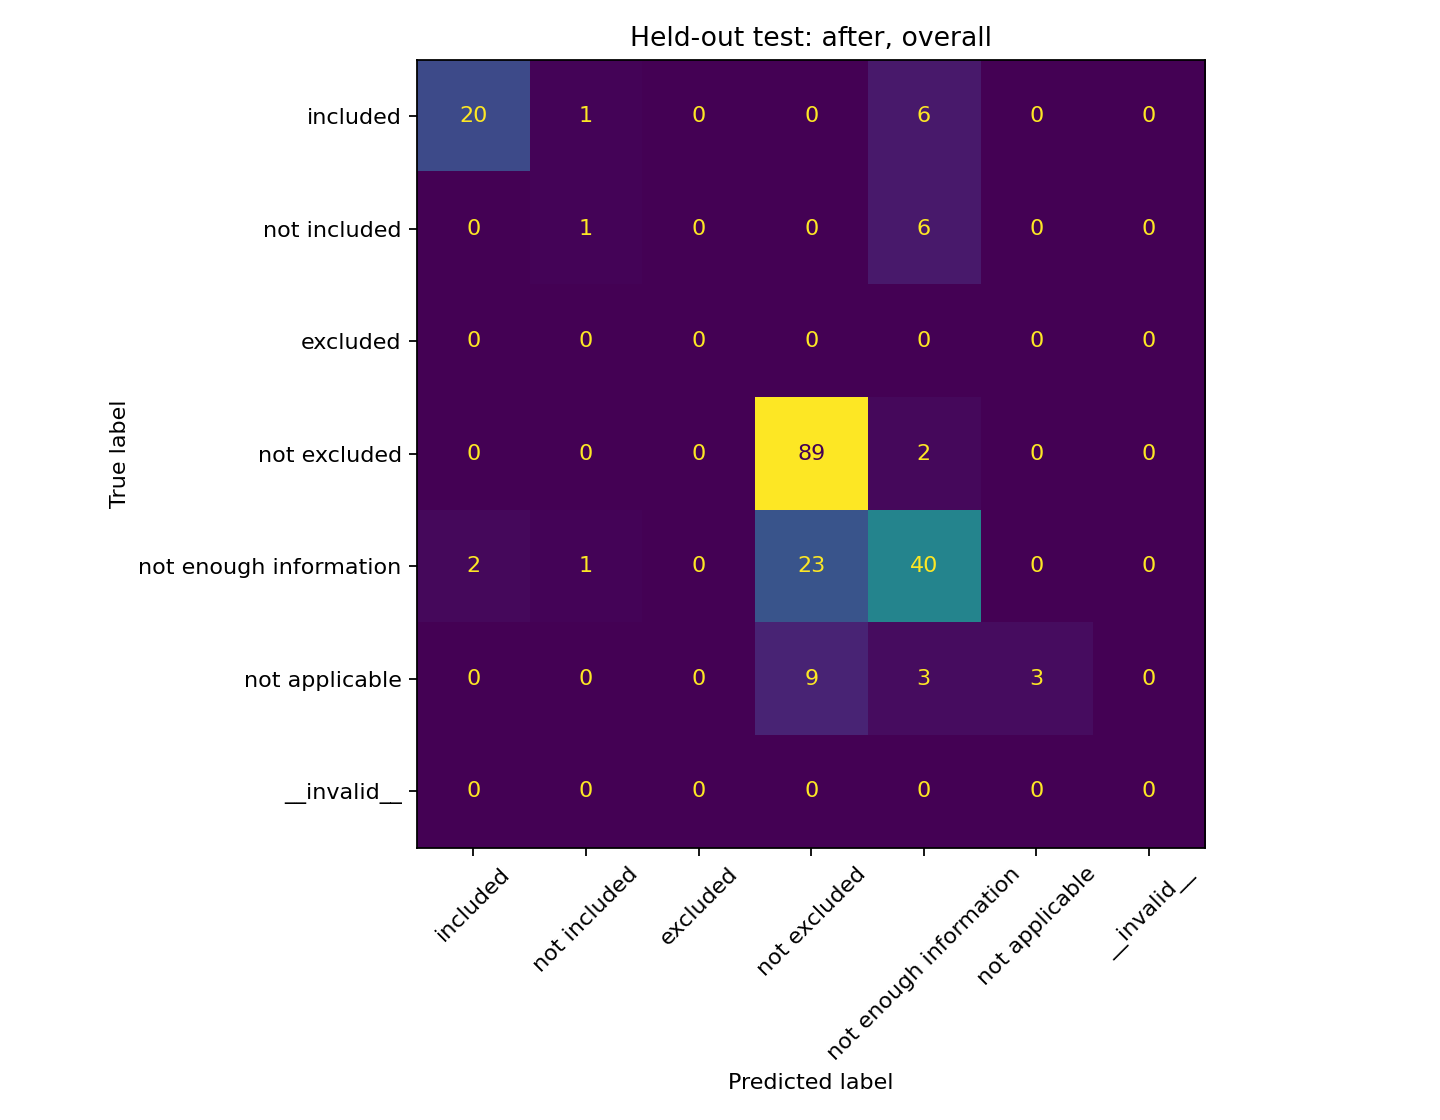
\includegraphics[width=\columnwidth]{../results/final_test/confusion_after_overall.png}\caption{Selected model's final held-out confusion matrix. Sparse/absent categories and remaining missing-information errors constrain interpretation.}\label{fig:testconfusion}\end{figure}
Figure~\ref{fig:testconfusion} visualizes these remaining errors. The eight examples in the later error-analysis section are drawn from these completed held-out predictions, after every model and prompt choice was fixed; they are analyzed for reporting, not fed back into training.
